\documentclass{beamer}
\mode<presentation>
{
\usetheme{Darmstadt}
%\usecolortheme{crane} %yellow
%%% BYU colored theme
\definecolor{BYUBlue}{RGB}{00,22,55}
\definecolor{BYUTan}{RGB}{232,211,175}
\usecolortheme[named=BYUBlue]{structure}
\setbeamercolor*{palette primary}{use=structure,fg=BYUBlue,bg=lightgray}
\setbeamercolor*{palette quaternary}{fg=white,bg=lightgray!0!BYUBlue}
\setbeamercolor{frametitle}{fg=BYUBlue,bg=BYUBlue!10}
\setbeamertemplate{items}[circle]
\setbeamertemplate{blocks}[rounded][shadow=True]
\setbeamertemplate{navigations symbols}{circle}
}

\usepackage{graphics}
\usepackage[english]{babel}
\usepackage[utf8]{inputenc}
\usepackage{times}
\usepackage[T1]{fontenc}
\usepackage{array}
\usepackage{amsmath,amssymb}
\usepackage{colortbl}
\usepackage{listings}
\usepackage{array}
\usepackage{threeparttable}
\usepackage{multirow}
\usepackage{amsthm}
\usepackage{float,graphicx,color}
\usepackage{graphics}
\usepackage{multicol}
\usepackage{natbib}
\usepackage{color}
\usepackage{hyperref}
\hypersetup{colorlinks, urlcolor=blue}
\usepackage{threeparttable}
\usepackage[format=hang,font=normalsize,labelfont=bf]{caption}
\usepackage{subcaption}
\usepackage{delarray}
\usepackage{amssymb}
\usepackage{setspace}
%\usepackage[pdftex]{graphicx}
\usepackage{placeins}
\usepackage{multirow}
\usepackage{mathtools}
\usepackage{animate}
\usepackage{bm}
\newcommand\ve{\varepsilon}
\newcommand\norm[1]{\left\lVert#1\right\rVert}

\title[Short Proposal Title]{\textbf{Full Proposal Title: \\ with Sweet Colon Style}}

%\subtitle
%{} % (optional)

\author[Evans]{\textbf{Dr. Richard W. Evans}}
% - Use the \inst{?} command only if the authors have different
%   affiliation.

\date[Short Occasion]{MACSS Project Proposal \\ April 4, 2018}

% This section of code puts a slide showing where you are in the outline
% at the beginning of each section
% \AtBeginSection[]
% {
%  \begin{frame}<beamer>{Outline}
%   \tableofcontents[currentsection]
%   %\tableofcontents[currentsection, subsection]
%  \end{frame}
% }


% If you wish to uncover everything in a step-wise fashion, uncomment
% the following command:

%\beamerdefaultoverlayspecification{<+->}


\begin{document}

\begin{frame}
  \titlepage
\end{frame}


\section{Intro}

  \begin{frame}
    \frametitle{Introduction}
    \begin{itemize}
      \item You might want to make a bulletted list
      \vspace{3mm}
      \item Remember to make your research question prominent early on in this section
    \end{itemize}
    \vspace{5mm}
    \begin{block}{Or you might want...}
      ...to use the block object to highlight something in a blue box
    \end{block}
    \vspace{5mm}
    \begin{alertblock}{Or you might want...}
      ...to use the alert block object to highlight something in a red box
    \end{alertblock}
  \end{frame}


\section{Theory}

  \begin{frame}
    \frametitle{Theory}
    \begin{itemize}
      \item State what theory you use
      \vspace{2mm}
      \item Maybe cite some key literature
      \vspace{2mm}
      \item Equations are helpful
      \footnotesize{\begin{equation*}
        \begin{split}
          &w_t e_{j,s}\bigl(1 - \tau^{mtrx}_{s,t}\bigr)(c_{j,s,t})^{-\sigma} = e^{g_y(1-\sigma)}\chi^n_{s}\biggl(\frac{b}{\tilde{l}}\biggr)\biggl(\frac{n_{j,s,t}}{\tilde{l}}\biggr)^{\upsilon-1}\Biggl[1 - \biggl(\frac{n_{j,s,t}}{\tilde{l}}\biggr)^\upsilon\Biggr]^{\frac{1-\upsilon}{\upsilon}} \\
          &\qquad\qquad\qquad\qquad\qquad\qquad\qquad\qquad\forall j,t, \quad\text{and}\quad E+1\leq s\leq E+S \\
        \end{split}
      \end{equation*}}
    \end{itemize}
  \end{frame}


\subsection{Data}

  \begin{frame}
  \frametitle{Data}
    \begin{itemize}
      \item In your data section you will want...
      \begin{itemize}
        \item a table of descriptive statistics
        \item some figures describing key properties of the data
      \end{itemize}
    \end{itemize}
  \end{frame}

  \begin{frame}
  \frametitle{Data Figure}
    \begin{figure}[htb]\centering
    \fbox{\resizebox{3.5in}{2.7in}{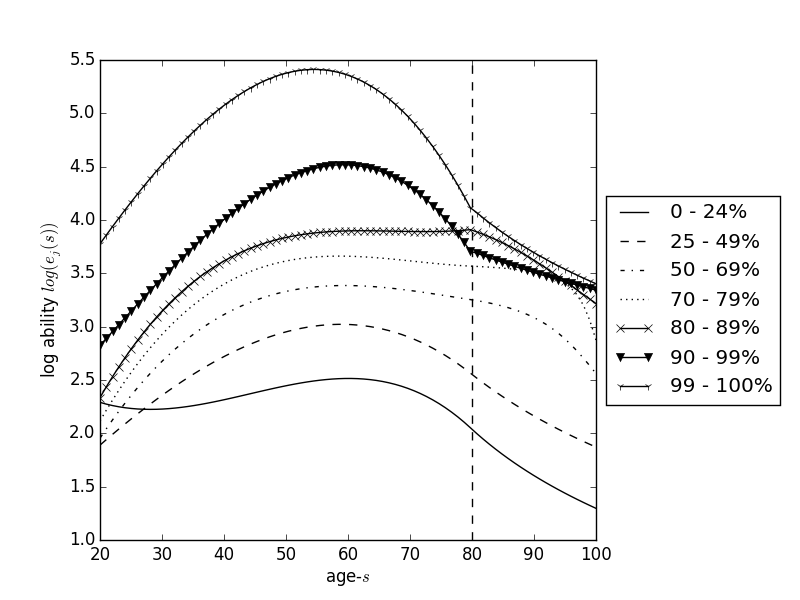
\includegraphics{images/ability_log_2D.png}}}
    \end{figure}
  \end{frame}

  \begin{frame}
  \frametitle{Data Table}
    \begin{threeparttable}
    \begin{tabular}{>{\scriptsize}l |>{\scriptsize}c >{\scriptsize}c >{\scriptsize}c >{\scriptsize}c}
      \hline\hline
      \textbf{Current Law} & Kids = 0 & Kids = 1 & Kids = 2 & Kids $\geq$ 3 \\
      \hline
      Maximum EITC        & \$510 & \$3,400 & \$5,616 & \$6,318 \\[-1mm]
      phase-in rate       & 0.0765 & 0.34 & 0.40 & 0.45 \\[-1mm]
      phase-out rate      & 0.0765 & 0.1598 & 0.2106 & 0.2106 \\[-1mm]
      phase-out start inc. & \$8,340 & \$18,340 & \$18,340 & \$18,340 \\[-1mm]
      \hline
      & Phase-out start & Min. age & Max. age & Max. disqual. \\[-2mm]
      & for married & for kids=0 & for kids=0 & investment \\[-2mm]
      & filing jointly & eligible & eligible & income \\[-1mm]
      & \$5,590 & 25 & 64 & \$3,450 \\[-1mm]
      \hline\hline
      \textbf{GAIN Act} & Kids = 0 & Kids = 1 & Kids = 2 & Kids $\geq$ 3 \\
      \hline
      Maximum EITC        & \cellcolor{yellow}\$3,000 & \cellcolor{yellow}\$6,528 & \cellcolor{yellow}\$10,783 & \cellcolor{yellow}\$12,131 \\[-1mm]
      phase-in rate       & \cellcolor{yellow}0.3 & \cellcolor{yellow}0.6258 & \cellcolor{yellow}0.768 & \cellcolor{yellow}0.864 \\[-1mm]
      phase-out rate      & \cellcolor{yellow}0.1598 & 0.1598 & 0.2106 & 0.2106 \\[-1mm]
      phase-out start inc. & \cellcolor{yellow}\$18,340 & \$18,340 & \$18,340 & \$18,340 \\[-1mm]
      \hline
      & Phase-out start & Min. age & Max. age & Max. disqual. \\[-2mm]
      & for married & for kids=0 & for kids=0 & investment \\[-2mm]
      & filing jointly & eligible & eligible & income \\[-1mm]
      & \$5,590 & \cellcolor{yellow} 21 & 64 & \$3,450 \\[-1mm]
      \hline\hline
    \end{tabular}
    \begin{tablenotes}
      \scriptsize{\item[]Note: Colored cells represent proposed changes.}
    \end{tablenotes}
    \end{threeparttable}
  \end{frame}


\section{Results}

  \begin{frame}
  \frametitle{Results}
    \begin{itemize}
      \item Put your analysis and results in this section
      \vspace{5mm}
      \item You will obviously not have much for this in your proposal presentation
      \vspace{5mm}
      \item This section will be benefit from both tables and figures
    \end{itemize}
  \end{frame}


\section{Conclusion}

  \begin{frame}
    \frametitle{Summary}
    \begin{itemize}
      \item Summarize your results
      \vspace{5mm}
      \item List any weaknesses of your model
      \vspace{5mm}
      \item List any future directions of research
    \end{itemize}
  \end{frame}


\end{document}

